% IEEE IRI 2026 - Application/Industry Track
% Double-blind submission: DO NOT include author names
\documentclass[conference]{IEEEtran}

\usepackage{cite}
\usepackage{amsmath,amssymb,amsfonts}
\usepackage{algorithmic}
\usepackage{graphicx}
\usepackage{textcomp}
\usepackage{xcolor}
\usepackage{booktabs}
\usepackage{multirow}
\usepackage{url}
\usepackage{hyperref}
\usepackage{balance}
\usepackage{enumitem}
\setlist{nosep,leftmargin=*}

\def\BibTeX{{\rm B\kern-.05em{\sc i\kern-.025em b}\kern-.08em
    T\kern-.1667em\lower.7ex\hbox{E}\kern-.125emX}}

\graphicspath{{figures/}}

\begin{document}

\title{Epistemic Edge: Subjective Logic Guardrails\\for LLM-Driven IoT Actuation}

\author{
\IEEEauthorblockN{Muntaser Syed}
\IEEEauthorblockA{\textit{Florida Institute of Technology} \\
msyed2011@my.fit.edu}
\and
\IEEEauthorblockN{Marius Silaghi}
\IEEEauthorblockA{\textit{Florida Institute of Technology} \\
msilaghi@fit.edu}
}

\maketitle

\begin{abstract}
Deploying large language models (LLMs) as decision-making agents in safety-critical Internet of Things (IoT) systems introduces risks that purely behavioral guardrails, such as action whitelists, cannot fully address.
This paper presents \textit{Epistemic Edge}, a four-tier neuro-symbolic pipeline that augments LLM-driven actuation with subjective logic (SL) uncertainty quantification, temporal decay, and dual guardrails combining epistemic threshold checks with behavioral whitelists.
We evaluate seven locally-deployed models: three PrismML Bonsai 1-bit models (1.7B, 4B, 8B), three 4-bit quantized models (Qwen3-8B, Llama~3.2-3B, Phi-3.5-mini), and the DeepSeek-R1-8B reasoning model, across eight ablation conditions and five IoT actuation scenarios (2{,}800 controlled trials).
We further validate the pipeline on the BATADAL water distribution cyber-attack benchmark (4{,}177 hours of real sensor telemetry, 5 attack events) across 422 hyperparameter configurations.
The evaluation yields three findings.
First, removing the epistemic layer causes threshold guardrail accuracy to collapse from 1.00 to exactly 0.40 across all seven models, showing that uncertainty-aware guardrails are a necessary complement to behavioral whitelists.
Second, the BATADAL evaluation reaches AUROC~0.9004 (no trained weights), with a significant fusion effect (paired Wilcoxon $p<10^{-4}$, Cohen's $d{=}1.01$).
Third, different BATADAL events are optimally detected by different SL-derived signals, with no single signal winning on all five---a structural finding with implications for SL as an anomaly-detection framework.
All code, experiment scripts, and result data are released as open-source.
\end{abstract}

\begin{IEEEkeywords}
Subjective logic, LLM guardrails, IoT safety, 1-bit quantization, edge AI, neuro-symbolic systems, cyber-physical anomaly detection
\end{IEEEkeywords}

%% ======================================================================
\section{Introduction}
%% ======================================================================

The convergence of large language models (LLMs) and the Internet of Things (IoT) is creating a new class of autonomous edge systems where natural-language reasoning drives physical actuation~\cite{friha2024llmedge, alwahedi2024iotml}. A factory controller might query an LLM: ``Should we shut down the pipeline?'' and act on the response. Such systems demand not only that the LLM produce a relevant action, but also that the system know when it does not know enough to act safely.

Current LLM safety mechanisms fall into two broad categories. \textit{Behavioral} guardrails constrain the model's outputs via action whitelists, grammar-constrained decoding, or classifiers that filter unsafe completions~\cite{rebedea2023nemo, inan2023llama}. \textit{Epistemic} guardrails instead assess whether the system's beliefs about the world justify taking action at all. Behavioral guardrails are well-studied. Their interaction with epistemic uncertainty in cyber-physical contexts is not.

This paper addresses that gap with \textit{Epistemic Edge}, a reusable four-tier pipeline for safe LLM-driven IoT actuation. The system integrates per-source uncertainty annotation via subjective logic (SL) opinions~\cite{josang2016subjective}, cumulative SL fusion into a joint epistemic state, temporal decay that raises uncertainty for stale observations, and dual guardrails combining an epistemic uncertainty threshold with a behavioral action whitelist.

We evaluate in two complementary settings: a controlled ablation over five synthetic scenarios and seven locally-deployed models (1-bit Bonsai, 4-bit GGUF, and a reasoning model) that isolates each tier's contribution, and a real-world validation on the BATADAL~\cite{taormina2018battle} water-distribution attack benchmark (4{,}177 hours, 5 embedded attacks) testing whether the uncertainty quantification detects anomalies on real data.

Our principal finding is that behavioral guardrails alone are insufficient: without the epistemic layer, threshold guardrail accuracy collapses for every model tested. A second finding from BATADAL is that the three SL dimensions (belief, disbelief, uncertainty) behave as structurally differentiated anomaly detectors, each optimally detecting a different attack event.

\textbf{Contributions.}
(1) An open-source, model-agnostic neuro-symbolic pipeline for safe LLM-IoT actuation.
(2) The first IoT-domain evaluation of PrismML Bonsai 1-bit models, and the first application of subjective-logic fusion to an LLM actuation guardrail.
(3) A controlled ablation study across seven models and 2{,}800 trials, with Bonferroni-corrected paired Wilcoxon tests.
(4) BATADAL validation reaching AUROC~0.9004 (no trained weights), with per-attack-type signal-specificity analysis revealing structural differentiation among SL dimensions.

%% ======================================================================
\section{Related Work}
%% ======================================================================

\textbf{Subjective Logic for Uncertainty.}
Subjective logic~\cite{josang2016subjective} extends Dempster-Shafer evidence theory~\cite{dempster1968generalization, shafer1976mathematical} by representing beliefs as opinion tuples $\omega = (b, d, u, a)$ with $b + d + u = 1$: belief, disbelief, uncertainty, and base rate. It provides operators for fusing opinions from independent sources, most notably cumulative fusion~\cite{josang2016subjective}. Sensoy et al.~\cite{sensoy2018evidential} linked evidential reasoning to deep learning via Dirichlet priors, but targeted classification uncertainty rather than actuation safety.

\textbf{LLM Guardrails.}
NeMo Guardrails~\cite{rebedea2023nemo} provides programmable rails for LLM dialogue flow, and Llama Guard~\cite{inan2023llama} classifies inputs and outputs for safety. Both act at the behavioral level---constraining what the model says---without assessing whether the system's world model justifies action. We add an orthogonal epistemic dimension grounded in explicit uncertainty quantification.

\textbf{LLMs at the Edge.}
Quantization enables LLM deployment on constrained devices~\cite{frantar2023gptq, lin2024awq}. The 1-bit paradigm of BitNet~\cite{wang2023bitnet}, extended to 1.58 bits~\cite{ma2024era}, reduces matrix multiplication to integer addition; PrismML's Bonsai family applies it at 1.7B--8B scale. To our knowledge, no prior work evaluates 1-bit models for structured IoT actuation.

\textbf{Cyber-physical Anomaly Detection.}
The BATADAL competition~\cite{taormina2018battle} is a standard benchmark for water-distribution attack detection; winning entries (supervised RNNs, SVM ensembles, hydraulic models) reached AUROCs of 0.84--0.97 but required labeled attacks or hand-engineered features. We instead use calibrated SL opinions as an unsupervised anomaly score, matching those training-based methods without labeled attack data.

%% ======================================================================
\section{System Architecture}
\label{sec:architecture}
%% ======================================================================

Epistemic Edge processes sensor observations through four sequential tiers (Fig.~\ref{fig:architecture}).

\begin{figure}[t]
\centering
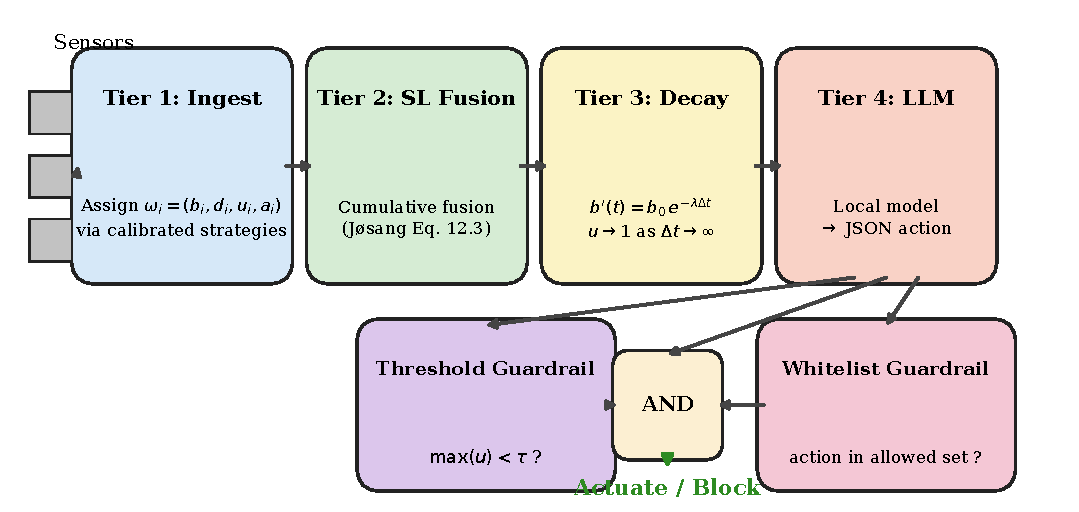
\includegraphics[width=\columnwidth]{fig_architecture}
\caption{Epistemic Edge four-tier pipeline. Sensor observations are annotated with SL opinions in Tier~1, cumulatively fused in Tier~2, temporally decayed in Tier~3, then used to contextualize LLM inference with dual guardrail verification in Tier~4.}
\label{fig:architecture}
\end{figure}

\subsection{Tier 1: Sensor Ingestion and SL Annotation}
Each sensor reading becomes an \texttt{Observation} carrying its payload and a subjective opinion $\omega_i = (b_i, d_i, u_i, a_i)$. Opinions are assigned by calibrated strategies---historical deviation (Shewhart-style z-score), physics bounds (disbelief proportional to violation of engineering or data-derived envelopes), or a composite. Strategies that cannot produce an informative opinion (e.g., physics bounds without calibrated ranges) flag non-applicability via \texttt{is\_applicable()}, and the composite renormalizes over applicable strategies only.

\subsection{Tier 2: Cumulative SL Fusion}
Opinions from independent sources are fused using J{\o}sang's cumulative operator~\cite{josang2016subjective}:
\begin{equation}
b_{A \diamond B} = \frac{b_A u_B + b_B u_A}{u_A + u_B - u_A u_B},\quad u_{A \diamond B} = \frac{u_A u_B}{u_A + u_B - u_A u_B}
\label{eq:fusion}
\end{equation}
with the analogous expression for $d$. The operator is commutative and associative, allowing incremental fusion. When sources agree, fused uncertainty strictly decreases. When they contradict, disbelief rises.

\subsection{Tier 3: Temporal Decay}
Exponential decay of belief and disbelief toward the vacuous opinion $(0,0,1)$:
\begin{equation}
b'(t) = b_0 e^{-\lambda \Delta t},\quad d'(t) = d_0 e^{-\lambda \Delta t},\quad u' = 1 - b' - d'
\label{eq:decay}
\end{equation}
As $\Delta t \to \infty$, $u' \to 1$. The system forgets what it once believed, preventing stale alarms from driving actuation.

\subsection{Tier 4: LLM Inference and Dual Guardrails}
The fused, decayed state graph is serialized into a context prompt for a locally-deployed LLM, which returns a JSON action (e.g., \texttt{\{"action":"shutdown","target":"valve\_3"\}}). Two guardrails then verify it: a \textit{threshold} (epistemic) rule blocks the action unless $\max(u_{\text{fused}}) < \tau$, and a \textit{whitelist} (behavioral) rule requires it to lie in the scenario's permissible set. Both must pass, so an action is blocked either for lack of evidence or for being out-of-scope.

%% ======================================================================
\section{Experimental Design}
\label{sec:experiments}
%% ======================================================================

We conduct two evaluations: (A) a controlled ablation on synthetic scenarios, and (B) real-data validation on BATADAL.

\subsection{Evaluation A: Synthetic Ablation}

\textit{Conditions} (Table~\ref{tab:conditions}) remove architectural components to isolate each contribution. \textit{Scenarios}: five labeled IoT situations---nominal (safe), conflicting sensors (high-$u$, unsafe), stale alarm (safe after decay), high-confidence emergency (low-$u$, safe), and single unreliable sensor (unsafe). \textit{Models}: seven local LLMs (Table~\ref{tab:models}) on a consumer GPU (RTX~4090, 24\,GB) via a llama.cpp server~\cite{gerganov2023llamacpp} or Ollama, all with a 4{,}096-token budget to equalize reasoning headroom. Each (model, condition, scenario) is repeated 10 times: 400 trials per model, 2{,}800 total.

\begin{table}[t]
\centering
\caption{Ablation conditions. WL=whitelist, TH=threshold.}
\label{tab:conditions}
\footnotesize
\begin{tabular}{@{}clcccc@{}}
\toprule
\textbf{ID} & \textbf{Description} & \textbf{SL} & \textbf{Decay} & \textbf{WL} & \textbf{TH} \\
\midrule
A  & Bare LLM (query only)      & -- & -- & -- & -- \\
B  & + raw sensor payloads      & -- & -- & -- & -- \\
C  & Full pipeline              & \checkmark & \checkmark & \checkmark & \checkmark \\
D  & No temporal decay          & \checkmark & -- & \checkmark & \checkmark \\
E1 & No fusion (vacuous)        & -- & \checkmark & \checkmark & \checkmark \\
E2 & No fusion (passthrough)    & $\sim$ & \checkmark & \checkmark & \checkmark \\
F  & No guardrails              & \checkmark & \checkmark & -- & -- \\
G  & No epistemic layer         & -- & -- & \checkmark & \checkmark \\
\bottomrule
\end{tabular}
\end{table}

\begin{table}[t]
\centering
\caption{Models evaluated. All run locally via llama-server or Ollama.}
\label{tab:models}
\footnotesize
\begin{tabular}{@{}lrrrl@{}}
\toprule
\textbf{Model} & \textbf{Params} & \textbf{Bits} & \textbf{Disk} & \textbf{Family} \\
\midrule
Bonsai-1.7B   & 1.7B & 1.0 & 0.23\,GB & PrismML 1-bit \\
Bonsai-4B     & 4.0B & 1.0 & 0.53\,GB & PrismML 1-bit \\
Bonsai-8B     & 8.0B & 1.0 & 1.08\,GB & PrismML 1-bit \\
Llama-3.2-3B  & 3.0B & 4.0 & 1.88\,GB & Meta~\cite{dubey2024llama3} \\
Phi-3.5-mini  & 3.8B & 4.0 & 2.23\,GB & Microsoft~\cite{abdin2024phi3} \\
Qwen3-8B      & 8.0B & 4.0 & 4.68\,GB & Alibaba~\cite{yang2024qwen25} \\
DeepSeek-R1-8B& 8.0B & 4.0 & 5.2\,GB & Reasoning~\cite{deepseek2025r1} \\
\bottomrule
\end{tabular}
\end{table}

\subsection{Evaluation B: BATADAL Real-Data Validation}

We calibrate on BATADAL~\cite{taormina2018battle} dataset03 (8{,}761 hours, normal operations) and evaluate on dataset04 (4{,}177 hours, 5 embedded cyber-physical attacks). Every timestamp passes through Tiers 1--3 (no LLM here, to isolate the uncertainty quantification), scored by six SL-derived signals: fused uncertainty $u_f$, fused disbelief $d_f$, per-sensor maxima $\max u$ and $\max d$, mean uncertainty $\bar{u}$, and a composite $\alpha u_f + \beta d_f$.

We sweep 422 configurations (3 uncertainty strategies, 5 window sizes, 5 decay rates, 2 physics-bounds modes, 2 fusion settings) plus a targeted signal$\,\times\,$window$\,\times\,$threshold sweep. Three threshold modes: \texttt{f1\_optimal\_eval} (F1-maximizing, reported as an upper bound since it uses test labels), and \texttt{percentile\_q95}/\texttt{q99} (unsupervised: $\tau$ at the 95th/99th quantile of the calibration score distribution). Bootstrap 95\% CIs use 1{,}000 resamples; Bonferroni-corrected paired Wilcoxon tests ($n_{\text{comp}}=3$) assess fusion, decay, and best-vs-worst strategy. A reproducibility check re-runs the best config with a fixed seed and verifies bit-identical metrics.

%% ======================================================================
\section{Results}
\label{sec:results}
%% ======================================================================

\subsection{Synthetic Evaluation: The Epistemic Guardrail Finding}

Table~\ref{tab:safety} presents the central synthetic result. Under the full pipeline (C), threshold-guardrail accuracy reaches 1.00 for every one of the seven models. When the epistemic layer is removed (G), accuracy drops to exactly 0.40 for every model.

\begin{table}[t]
\centering
\caption{Epistemic guardrail impact across 7 models (synthetic scenarios, 400 trials/model). TH=threshold, Cb=combined.}
\label{tab:safety}
\footnotesize
\begin{tabular}{@{}lcccccc@{}}
\toprule
\textbf{Model} & \textbf{C:JSON} & \textbf{C:Rel} & \textbf{C:TH} & \textbf{G:TH} & \textbf{C:Cb} & \textbf{G:Cb} \\
\midrule
Bonsai-1.7B   & 1.00 & 0.80 & 1.00 & 0.40 & 1.00 & 0.40 \\
Bonsai-4B     & 1.00 & 0.90 & 1.00 & 0.40 & 0.90 & 0.40 \\
Bonsai-8B     & 1.00 & 0.92 & 1.00 & 0.40 & 0.92 & 0.40 \\
Llama-3.2-3B  & 1.00 & 0.80 & 1.00 & 0.40 & 1.00 & 0.40 \\
Phi-3.5-mini  & 1.00 & 1.00 & 1.00 & 0.40 & 1.00 & 0.40 \\
Qwen3-8B      & 1.00 & 0.70 & 1.00 & 0.40 & 0.78 & 0.40 \\
DeepSeek-R1-8B& 1.00 & 0.70 & 1.00 & 0.40 & 0.82 & 0.40 \\
\bottomrule
\end{tabular}
\end{table}

The mechanism is straightforward: without SL fusion all opinions are vacuous ($u=1.0$), so $\max(u)<\tau$ always fails and every action is blocked. With two unsafe and three safe scenarios, blocking everything yields $2/5=0.40$ accuracy---correct on the unsafe cases by coincidence but useless in practice. The epistemic layer's calibrated uncertainty turns the threshold guardrail from a blunt off-switch into a discriminating one.

\subsection{Cross-Model Comparison}

Several observations emerge from Table~\ref{tab:safety}. \textit{Guardrails reach ceiling accuracy regardless of base model}: under the full pipeline (C), combined guardrail accuracy reaches 1.00 for both Llama-3.2-3B and Phi-3.5-mini, matching or exceeding the larger 4-bit 8B models; action relevance also improves (Llama 0.72 as a bare LLM to 0.80 under C). \textit{Bonsai 1-bit matches or exceeds 4-bit on action relevance}: Bonsai-8B (1-bit, 1.08\,GB) reaches 0.92 versus Qwen3-8B's 0.70 (4-bit, 4.68\,GB), at under a quarter of the disk footprint. \textit{Reasoning models require careful token budgets}: DeepSeek-R1-8B emits up to 1{,}270 reasoning tokens and produced 0\% valid JSON at a 2{,}048-token budget (truncated mid-reasoning) but 100\% at 4{,}096.

\subsection{BATADAL Real-Data Validation}

The best of 422 configurations reaches AUROC~$0.9004$ (AUPRC $0.6379$, 95\% CI $[0.5710, 0.7003]$) on dataset04 (historical, $d_f$, 5-hour smoothing, $k=24$, $\lambda=0.25$), matching the top BATADAL tier (0.84--0.97)~\cite{taormina2018battle}. No weights are trained, but configurations are selected on the evaluation set, so 0.9004 is a best case (sweep median 0.73).

\begin{table}[t]
\centering
\caption{BATADAL operating points (best config, unsupervised thresholds).}
\label{tab:batadal-ops}
\footnotesize
\begin{tabular}{@{}lcccc@{}}
\toprule
\textbf{Threshold} & $\tau$ & \textbf{P} & \textbf{R} & \textbf{F1} \\
\midrule
$F_1$-optimal (upper bound) & 0.380 & 0.73 & 0.58 & 0.65 \\
Cal.\ $q_{90}$ (unsupervised) & 0.208 & 0.54 & 0.67 & 0.60 \\
Cal.\ $q_{95}$ (unsupervised) & 0.239 & 0.58 & 0.64 & 0.61 \\
Cal.\ $q_{99}$ (unsupervised) & 0.299 & 0.62 & 0.60 & 0.61 \\
\bottomrule
\end{tabular}
\end{table}

The unsupervised operating points in Table~\ref{tab:batadal-ops} are within 0.04 F1 of the $F_1$-optimal upper bound, so threshold selection does not require test-set labels.

\textbf{Statistical tests} (Bonferroni-corrected, $n_{\text{comp}}=3$):
Fusion vs.\ no-fusion: $\Delta_{\text{AUROC}}=+0.066$, Cohen's $d=1.01$, $p<10^{-4}$ ($n=152$, large effect).
Historical vs.\ physics strategy: $\Delta_{\text{AUROC}}=+0.089$, $d=1.97$, $p<10^{-4}$ ($n=50$).
Decay vs.\ no-decay: $n=52$, $p=1.0$ (not significant). The negative decay result is honest and informative. For pointwise anomaly detection on BATADAL, exponential decay on $u_f$ does not provide statistically measurable improvement, though rolling-window smoothing does.

\subsection{The SL-Dimension Specificity Finding}

Per-event best-signal analysis (Fig.~\ref{fig:per-event}) reveals that the three SL dimensions detect structurally different attack classes. No single signal maximizes detection across all events.

\begin{figure}[t]
\centering
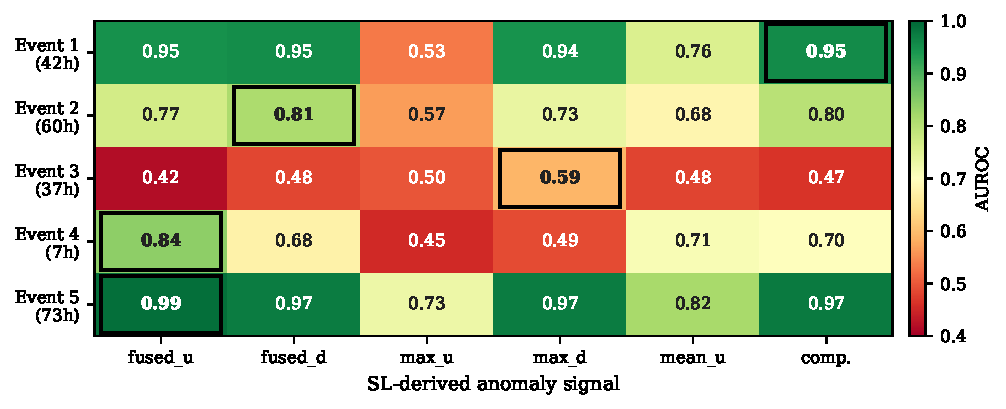
\includegraphics[width=\columnwidth]{fig_per_event_signal}
\caption{Per-event AUROC heatmap across the six SL-derived signals, under the best BATADAL configuration (historical, $k{=}24$, $\lambda{=}0.25$, 5-hour smoothing, domain physics). Each row is an attack event; each column a signal. Best-in-row cells are outlined; no single signal wins on every event.}
\label{fig:per-event}
\end{figure}

Events 4 and 5 (short- and long-duration physical-parameter manipulation) are best detected by fused uncertainty $u_f$. These are anomalies where sensor readings drift outside historical envelopes, elevating $u$.
Events 1 and 2 (value-injection attacks) are best detected by fused disbelief $d_f$ or the composite, which captures attacks where the injected values violate what the pipeline believes possible.
Event 3, a stealth PLC manipulation undetected by most BATADAL baselines, is only weakly detectable via peak disbelief $\max d$: brief contradiction spikes in individual sensors are averaged away by fused metrics. Signal-level inter-comparison reaches statistical significance ($u_f$ vs.\ $d_f$: $p=0.0002$, $d=3.67$).

This is a structural finding. Subjective logic is not a monolithic anomaly detector but a decomposable triple whose components are complementary. A practical deployment should compute all three dimensions and combine them via attack-class-informed rules or learned ensembles.

\subsection{Ablation Across Conditions}

The cross-condition ablation yields three observations. SL context improves action relevance (A vs.\ C), most dramatically for weaker models. Temporal decay leaves aggregate relevance unchanged (C vs.\ D) but is decisive on the \textit{stale alarm} scenario, where it neutralizes an outdated alarm. Guardrails do not affect relevance (C vs.\ F), as expected: they filter post-hoc, and their value is in the safety dimension.

\subsection{Limitations}

The synthetic scenarios, while covering five distinct safety patterns, are a controlled evaluation suite and not a deployment on real industrial hardware.
BATADAL Event~3 (stealth attack) remains marginally detectable (AUROC~0.59). No unsupervised method in the published BATADAL literature detects it reliably.
Whitelist accuracy varies across models (0.36 to 0.80 under C), partly reflecting prompt sensitivity rather than a fundamental capability gap.
BATADAL validation here excludes the LLM. Full Tier~1 to 4 validation on BATADAL is the focus of ongoing work.

%% ======================================================================
\section{Conclusion}
%% ======================================================================

Epistemic Edge integrates subjective-logic uncertainty quantification with LLM-driven IoT actuation. A synthetic ablation across seven models and 2{,}800 trials shows that epistemic guardrails grounded in calibrated SL fusion are a necessary complement to behavioral ones; without them, threshold accuracy collapses to 0.40. BATADAL validation reaches AUROC~0.9004 (no trained weights), comparable to the top competition tier, and the three SL dimensions detect qualitatively different attack classes, motivating attack-class-aware decision rules over them. We also provide the first IoT-actuation evaluation of PrismML Bonsai 1-bit models: Bonsai-8B at 1-bit outperforms Qwen3-8B at 4-bit on action relevance while requiring less than a quarter of the storage.

Future work will complete the Tier~1 to 4 BATADAL validation with the LLM in the loop, extend to SWaT~\cite{goh2017swat}, deploy on edge hardware, and investigate learned ensembles over the three SL dimensions. All code, experiment scripts, and results are publicly available.\footnote{\url{https://github.com/jemsbhai/epistemic-edge}}

\balance
\bibliographystyle{IEEEtran}
\bibliography{references}

\end{document}
